\documentclass[10pt]{beamer}

%  {{{ Handout Generation

% \documentclass[10pt,handout]{beamer}
% \usepackage{pgfpages}
% \pgfpagesuselayout{4 on 1}[a4paper, landscape, border shrink=5mm]
% \pgfpageslogicalpageoptions{1}{border code=\pgfusepath{stroke}}
% \pgfpageslogicalpageoptions{2}{border code=\pgfusepath{stroke}}
% \pgfpageslogicalpageoptions{3}{border code=\pgfusepath{stroke}}
% \pgfpageslogicalpageoptions{4}{border code=\pgfusepath{stroke}}

% }}}
% {{{ Packages

\usepackage{soul}
\usepackage{amsmath}
\usepackage{todonotes}
\usepackage{graphicx}
\usepackage{xcolor}
\usepackage{pgfplots}
\usepackage{tikz}
\usetikzlibrary{shapes}
\usetikzlibrary{math}
\usetikzlibrary{patterns}
\usetikzlibrary{shapes,arrows,positioning,decorations.markings}
\usetikzlibrary{decorations.pathmorphing, decorations.text}
\usepackage[no-math]{fontspec}
% \usepackage{fontawesome}
% \newfontfamily{\FA}{FontAwesome}

\definecolor{KTHBlue}{HTML}{003C9E}
\definecolor{DarkGreen}{HTML}{526B0B}
\definecolor{DarkRed}{HTML}{AB2511}
\definecolor{DarkOrange}{HTML}{D16415}

% }}}
% {{{ Theming
\usetheme[progressbar=frametitle]{metropolis}

\setbeamercolor{normal text}{%
	fg=black!90,
	bg=black!2
}
\setbeamercolor{alerted text}{%
	fg=KTHBlue!80,
	bg=black!2
}
\setbeamercolor{palette primary}{%
	use=normal text,
	fg=normal text.bg,
	bg=KTHBlue
}
\setbeamercolor{progress bar in head/foot}{fg=KTHBlue, bg=KTHBlue!10}
\setbeamercolor{progress bar in section page}{fg=KTHBlue, bg=KTHBlue!10}
\setbeamercolor{title separator}{fg=KTHBlue}

\AtBeginSubsection{\frame{\subsectionpage}}


% }}}
% {{{ Title Page

\title{HDF5}
\subtitle{Métadonnées et compression pour grosses données}
\author{Mathieu Gaborit}
\date{Human Talks -- La Ruche Numérique -- Oct. 2017}
\institute{}
\titlegraphic{\begin{tikzpicture}[overlay]
	\draw (7.8,-8.0) node {
\includegraphics[height=.9cm]{imgs/logos/ruche.png}};%
	\draw (10.,-8.0) node {
\includegraphics[height=.9cm]{imgs/logos/haum.png}};%
	\end{tikzpicture}
}

% }}}
% {{{ Custom Command

\newcommand\cRed{\textcolor{DarkRed}}
\newcommand\cBlue{\textcolor{KTHBlue}}
\newcommand\cGreen{\textcolor{DarkGreen}}
\newcommand\cOrange{\textcolor{DarkOrange}}

\newcommand\etc{\textit{etc.}}
\newcommand\mbf{\mathbf}
\newcommand\dd{\mathsf{d}}
\newcommand\ff{\mathbf{f}}
\newcommand\FF{\mathbf{F}}
\newcommand\RR{\mathbf{R}}
\newcommand\bS{\mathbf{S}}
\newcommand\QQ{\mathbf{Q}}
\newcommand\DD{\mathcal{D}}
\newcommand\ZZ{\mathbb{Z}}
\newcommand\PP{\mathbb{P}}

\newcommand{\btVFill}{\vskip0pt plus 1filll}

% }}}
% {{{ Graphics

\usepackage{minted}

\newminted{python}{fontsize=\scriptsize,
                   numbersep=8pt,
                   gobble=4,
                   framesep=3mm}

\newcommand\fileimage[1]{%
	\draw[fill=black!2] (#1) -- ++(2,0) -- ++(0,2.5) -- ++(-1.5,0) -- ++(-.5,-.5) -- cycle;
}

% }}}
\begin{document}

% {{{ Title and TOC
\maketitle

% \begin{frame}{Contenu}
% 	\setbeamertemplate{section in toc}[sections numbered]
% 	\tableofcontents[hideallsubsections]
% \end{frame}

\begin{frame}{\$ whoami}
	\begin{center}
		Mathieu (matael) Gaborit
	\end{center}

	\begin{itemize}
		\item Thésard au LAUM (Le Mans) \& au KTH (Stockholm)
		\item Co-fondateur du HAUM (\alert{haum.org})
		\item Co-fondateur de \alert{sample.cat} (un peu en stand-by malheureusement)
		\item Hacker, mangeur de données, curieux, \etc.
	\end{itemize}
\end{frame}

\begin{frame}[standout]
	On génère des données... Plein.

	\pause

	Parfois on les traite tout de suite,

	\pause
	souvent on revient dessus beaucoup plus tard.
\end{frame}

\begin{frame}{Quelque soit l'usage}

	\begin{itemize}
		\item expériences/manips
		\item simulations
		\item potager connecté
		\item logs
		\item \etc
	\end{itemize}

	\pause

	Deux points compliqués :

	\begin{itemize}
		\item ré-analyse après un long moment
		\item reproductibilité/conditions d'obtention
	\end{itemize}
\end{frame}

\begin{frame}{Réponses ?}
	\begin{block}{Conservation longue}
		Nécessité de compresser pour gagner de la place
	\end{block}

	\begin{block}{Ré-analyse \& Reproductibilité}
		Besoin de conserver des métas données
	\end{block}
\end{frame}

\begin{frame}{L'idée bidouille}
	\centering
	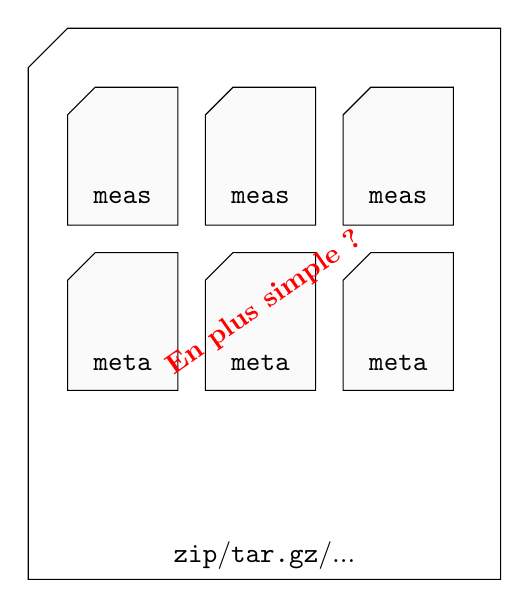
\begin{tikzpicture}

		\begin{scope}[scale=.7]
			\uncover<1->{
				\foreach \ii in {0,...,2} {
					\fileimage{2.5*\ii,0}
					\node (tmp) at (2.5*\ii+1,.5) {\texttt{meas}};
				}
			}


			\uncover<2->{
				\foreach \ii in {0} {
					\fileimage{2.5*\ii,-3}
					\node (tmp) at (2.5*\ii+1,-3+.5) {\texttt{meta}};
				}
			}

			\uncover<3->{
				\foreach \ii in {1,2} {
					\fileimage{2.5*\ii,-3}
					\node (tmp) at (2.5*\ii+1,-3+.5) {\texttt{meta}};
				}
			}
		\end{scope}

		\uncover<4->{
			\draw (-.5,-4.5) -- ++(6,0) node[midway, above] {\texttt{zip}/\texttt{tar.gz}/...} -- ++(0,7) -- ++(-5.5,0) -- ++(-.5,-.5) --cycle;
		}

		\uncover<5->{
			\node[red, rotate=35, anchor=center] (this) at (2.5, -1) {\textbf{En plus simple ?}};
		}
	\end{tikzpicture}
\end{frame}

\begin{frame}{HDF5}
	\begin{center}
		Hierarchical Data Format v5
	\end{center}

	\begin{itemize}
		\item orienté dataset
		\item hiérarchie (notion de groupes, sous-groupes, \etc)
		\item métadonnées sur tous les éléments
		\item compressions
	\end{itemize}
\end{frame}

\begin{frame}{Concrètement ?}
	\centering
	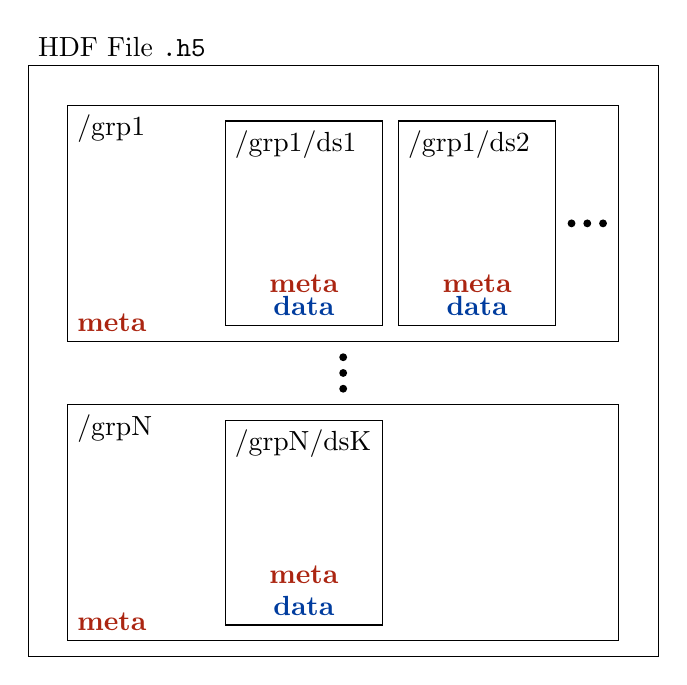
\begin{tikzpicture}
		\draw (0,-0.5) rectangle (8,7);
		\node[anchor=south west] (tmp) at (0,7) {HDF File \texttt{.h5}};

		\only<+->{
			\draw (.5,6.5) node[anchor=north west] {/grp1} rectangle ++(7,-3);
		}

		\only<+->{
			\draw (2.5,6.3) node[anchor=north west] {/grp1/ds1} rectangle ++(2,-2.6);
		}
		\only<+->{
			\draw (4.7,6.3) node[anchor=north west] {/grp1/ds2} rectangle ++(2,-2.6);

			\foreach \ii in {0,...,2}{
				\fill (6.9+\ii*0.2,5) circle (.05);
			}
		}

		\only<+->{
			\foreach \ii in {0,...,2}{
				\fill (4,3.3-\ii*0.2) circle (.05);
			}
			\draw (.5,2.7) node[anchor=north west] {/grpN} rectangle ++(7,-3);
			\draw (2.5,2.5) node[anchor=north west] {/grpN/dsK} rectangle ++(2,-2.6);
		}

		\only<+->{
			\foreach \xx/\yy in {3.5/3.7, 5.7/3.7, 3.5/-.1} {
				\node[anchor=south, KTHBlue] (tmp) at (\xx,\yy) {\textbf{data}};
			}
		}

		\only<+->{
			\foreach \xx/\yy/\anch in {3.5/4/south, 5.7/4/south, 3.5/.3/south, .5/3.5/{south west}, .5/-.3/{south west}} {
				\node[anchor=\anch, DarkRed] (tmp) at (\xx,\yy) {\textbf{meta}};
			}
		}
	\end{tikzpicture}
\end{frame}

\begin{frame}{Possibilités}
	\begin{itemize}
		\item Stockage de métadonnées au plus proche des données qu'elles décrivent
		\item Adressage depuis la racine ou en relatif (\texttt{/grp1/ds2} ou \texttt{ds2})
		\item Datasets à $n$ dimensions
		\item Compression
	\end{itemize}
\end{frame}


\begin{frame}[fragile]{Interface Python}

	\begin{itemize}
		\item Wrapper autour de la lib' C : \alert{h5py}
		\item Interface plus haut niveau : \alert{PyTables}
	\end{itemize}

\defverbatim[colored]\lstI{
	\begin{pythoncode}
    import h5py
    import numpy as np

    fh = h5py.File('fichier.h5', 'w')
    grp1 = fh.create_group('grp1')
    ds1 = grp1.create_dataset('ds1', data=np.ones(10,1))
    grp1.attrs['date'] = "aujourd'hui"
    ds1.attrs['type'] = 'uns'

    fh.close()

	\end{pythoncode}
}
\lstI

\begin{center}
	Rien de bien méchant :)
\end{center}
\end{frame}

\begin{frame}[fragile]{Interface Python}

\defverbatim[colored]\lstI{
	\begin{pythoncode}
    import h5py
    import numpy as np

    fh = h5py.File('fichier.h5', 'r')
		ds1 = fh['grp1']['ds1']
    ds1_bis = fh['/grp1/ds1']

    fh.close()

	\end{pythoncode}
}
\lstI
\end{frame}

\begin{frame}{Un monde parfait ?}
	Non...

	\begin{itemize}
		\item adapté aux données numériques
		\item mauvaise gestion des chaines (pas d'UTF8 par exemple)
		\item un seul gros fichier $\Rightarrow$ corruption!
		\item spécification horrible (150 pages) $\Rightarrow$ une seule implémentation
	\end{itemize}
\end{frame}

\begin{frame}{Du coup on fait quoi ?}
	Si vous avez des données :

	\begin{itemize}
		\item numériques
		\item complexes (besoin de métadata)
		\item grosses mais pas immenses
	\end{itemize}

	\begin{center}
		\textcolor{KTHBlue}{GO !}
	\end{center}

	Sinon... tant pis pour vous !
\end{frame}

\begin{frame}[standout] % Thank you
	% Thank you!\\
	\vspace{0.05\textwidth}
	Merci !\\
	\vspace{0.25\textwidth}
	\small{\texttt{mathieu@haum.org}}
\end{frame}

\end{document}
